\subsection{Функциональная структура компилятора}
\label{impl:compiler} % \index{Chapter7}

Используя знания о MLIR и DaVinci, полученные в результате исследовательской
работы, наша команда приступила к разработке нового компилятора. Было решено
создать новые диалекты, которые на разных уровнях абстракции отражают
особенности архитектуры DaVinci. Перечислим их и отметим основные особенности:

\begin{enumerate}
    \item ascend --- диалект крупноблочных операций. Является аналогом HLO, но
          операции в нём предъявляют требования к типам данных: матрицы должны
          быть расположены в блочном формате. Поэтому в процессе lowering-а
          из HLO в ascend для входных и выходных данных вставляются операции
          фрактализации, т.е. приведения матрицы к нужному виду. Для остальных
          диалектов требование на формат данных сохраняется, при этом считается,
          что оно выполняется благодаря корректности представления графа
          исполнения в диалекте ascend.

    \item cce --- диалект операций, схожих с ассемблерными инструкциями.
          Основная его особеннность заключается в сохранении семантики
          тензоров, что позволяет упрощать процесс генерации таких операций и
          их верификации (проверки корректности).

    \item hivm --- диалект непосредственных ассемблерных инструкций. Он в
          точности повторяет их семантику, что упрощает его ловеринг в llvm.
\end{enumerate}

Конвейер (пайплайн) компиляции для девайса выглядит следующим образом:

\begin{figure}[h!]
      \centering
      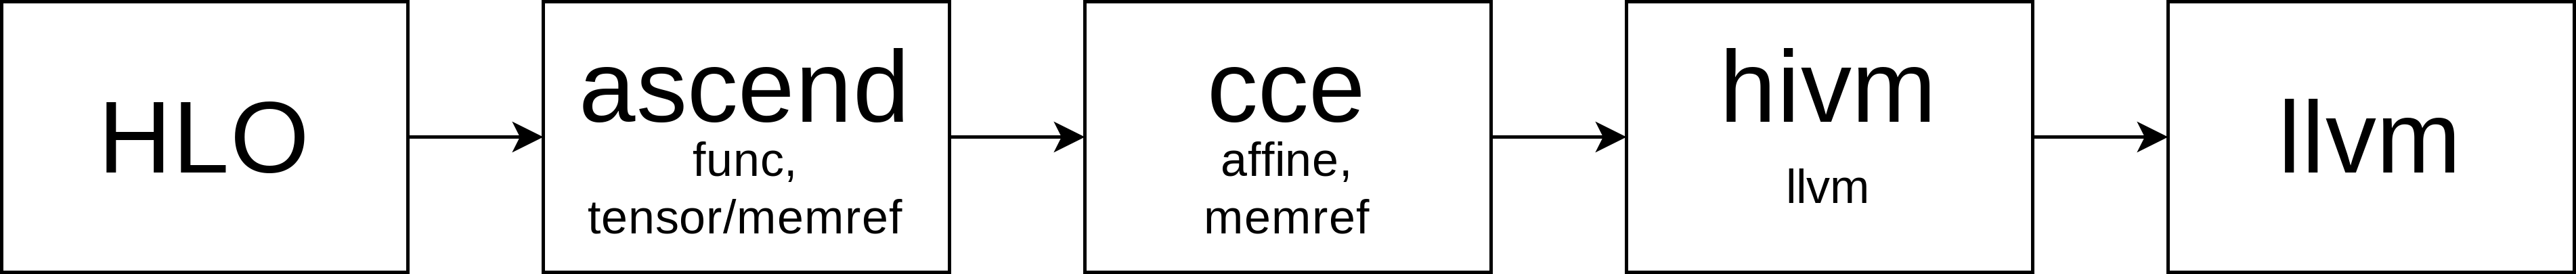
\includegraphics[scale=0.1]{Compiler.png}
      \caption{Пайплайн компиляции для девайса}
  \end{figure}
